\documentclass[12pt,a4paper]{report}
%
% This LaTeX template has been created by Luca Grilli
% Based on the following https://en.wikibooks.org/wiki/LaTeX/Title_Creation
%
\usepackage[italian]{babel}
\usepackage[T1]{fontenc}
\usepackage{geometry}
\usepackage{graphicx}
\usepackage{hyperref}
\usepackage[utf8]{inputenc}
\usepackage{lipsum} % genera testo fittizio
\usepackage{subcaption}
\usepackage[nottoc,numbib]{tocbibind}
\usepackage{titlesec}
\usepackage{xcolor}
\usepackage{listings}

% Stile per i listati di codice Java
\lstdefinestyle{java}{
  language=Java,
  basicstyle=\ttfamily\footnotesize,
  keywordstyle=\color{blue!70!black}\bfseries,
  commentstyle=\color{gray}\itshape,
  stringstyle=\color{teal},
  numbers=left,
  numberstyle=\tiny\color{gray},
  numbersep=8pt,
  showstringspaces=false,
  breaklines=true,
  frame=single,
  framesep=4pt,
  tabsize=4,
  captionpos=b,
  literate=%
    {à}{{\`a}}1 {è}{{\`e}}1 {é}{{\'e}}1 {ì}{{\`i}}1 {ò}{{\`o}}1 {ù}{{\`u}}1
}
\renewcommand{\lstlistingname}{Listato}

\titleformat{\chapter}[display]{\Huge\bfseries}{}{0pt}{\thechapter.\ }

\graphicspath{{figures/}}
%
%\addtolength{\topmargin}{-.875in} % reduce the default top margin
%\addtolength{\topmargin}{-2cm} % reduce the default top margin
%



%%%%%%%%%%%%%%%%%%%%%%%%%%%%%%%%%%
%                                %
%     Begin Docuemnt [start]     %
%                                %
%%%%%%%%%%%%%%%%%%%%%%%%%%%%%%%%%%
\begin{document}



%%%%%%%%%%%%%%%%%%%%%%%%%%%%%%
%     Title Page [start]     %
%%%%%%%%%%%%%%%%%%%%%%%%%%%%%%
% Declare new goemetry for the title page only.
\newgeometry{margin=1in}
\begin{titlepage}
	\centering
	
\includegraphics[width=0.34\textwidth]{logo-unipg}\par\vspace{1cm}
	\large{Tesina Finale di}\par
	\large{\textbf{Programmazione di Interfacce Grafiche e Dispositivi Mobili}}\par
	\small{Corso di Laurea in Ingegneria Informatica ed Elettronica -- A.A. 2025-2026}\par
	\textsc{\small{Dipartimento di Ingegneria}}\par
	%\large{A.A. 2018-2019}\par

	%\vfill
	\vspace{0.5cm}
	docente\par
	Prof.~Luca \textsc{Grilli}

	\vspace{1cm}
	%\textsc{\large{Tesina Finale a.a. 2018-2019}}\par
	\vspace{1cm}
	\textbf{\huge{Dragon Ball Z Fighting Game}}\par
	\vspace{0.2cm}
	applicazione desktop \textsc{JFC/Swing}\par
	%applicazione desktop \textsc{JavaFX}\par
	%app nativa per Android sviluppata con \textsc{AndroidStudio}\par
	\vspace{0.5cm}
	
\includegraphics[width=0.40\textwidth]{icon.png}\par\vspace{1cm}
	\vspace{1cm}

	%\begin{tabular}{ l l l l }
	%\Large{\emph{112233}} & \Large{\emph{Mario}} & \Large{\emph{Rossi}} & \Large{\emph{mario.rossi@studenti.unipg.it}}\\
	%\Large{\emph{114455}} & \Large{\emph{Carlo}} & \Large{\emph{Bianchi}} & \Large{\emph{carlo.bianchi@studenti.unipg.it}}\\
	%\end{tabular}

	\large{studente}\par
	\vspace{0.2cm}
	\begin{tabular}{ l l l l }
	\large{380286} & \large{\textbf{Leonardo}} & \large{\textbf{Alunno}} & \large{leonardo.alunno1@studenti.unipg.it}\\
	\end{tabular}

	%\begin{tabular}{ l l l l }
	%112233 & Mario & Rossi & mario.rossi@studenti.unipg.it\\
	%114455 & Carlo & Bianchi & carlo.bianchi@studenti.unipg.it\\
	%\end{tabular}

	\vfill
	% Bottom of the page
	%{\large \today\par}
	\raggedright
	\small{Data ultimo aggiornamento: \today}
\end{titlepage}
% Ends the declared geometry for the titlepage
\restoregeometry
%%%%%%%%%%%%%%%%%%%%%%%%%%%%
%     Title Page [end]     %
%%%%%%%%%%%%%%%%%%%%%%%%%%%%

%%%%%%%%%%%%%%%%%%%%%%%%%%
%     Indice [start]     %
%%%%%%%%%%%%%%%%%%%%%%%%%%
\tableofcontents
%%%%%%%%%%%%%%%%%%%%%%%%
%     Indice [end]     %
%%%%%%%%%%%%%%%%%%%%%%%%

%%%%%%%%%%%%%%%%%%%%%%%%%%%%%%%%%%%%%%%%%%%%
%     Descrizione del Problema [start]     %
%%%%%%%%%%%%%%%%%%%%%%%%%%%%%%%%%%%%%%%%%%%%
\chapter{Descrizione del Problema}\label{ch:despro}
L'obiettivo di questo lavoro è lo sviluppo di un'applicazione desktop consistente in un videogioco di combattimento bidimensionale (\emph{2D fighting game}) a due giocatori, ispirato alla serie \emph{Dragon Ball Z} e, in particolare, al titolo \emph{Dragon Ball Z: Extreme Butōden}~\cite{extremebutoden} per Nintendo 3DS.

L'applicazione è implementata utilizzando la tecnologia JFC/Swing, in modo da favorire un'ampia portabilità sui diversi sistemi operativi riducendo al minimo le modifiche al codice sorgente. Il codice è stato sviluppato e testato su piattaforma macOS, ma non fa uso di funzionalità specifiche del sistema operativo e risulta pertanto eseguibile su qualunque piattaforma dotata di Java Runtime Environment.

\medskip
Di seguito si fornisce una breve descrizione del genere \emph{fighting game} e del titolo che ha ispirato il progetto; successivamente si descrive l'applicazione che si intende realizzare.

%----------------------------------------------
% Sezione: Il genere fighting game [start]
%----------------------------------------------
\section{Il genere \emph{fighting game}}\label{se:fighting}
Il \emph{fighting game} (``picchiaduro'') è un genere videoludico in cui due personaggi si affrontano in un combattimento all'interno di un'arena delimitata. Ciascun giocatore controlla il proprio personaggio impartendo comandi di movimento e di attacco; l'obiettivo è ridurre a zero i punti vita (\emph{health points}) dell'avversario prima che questi faccia altrettanto. La profondità di gioco tipica del genere deriva dalla combinazione di attacchi in sequenza (\emph{combo}), dalla gestione di risorse accumulabili durante lo scontro e dalla componente strategica di attacco e difesa.

Il titolo di riferimento per questo progetto, \emph{Dragon Ball Z: Extreme Butōden}, appartiene al sottogenere dei picchiaduro bidimensionali a scorrimento, caratterizzati da una grafica \emph{pixel art}, da animazioni fluide e da un sistema di combattimento incentrato su combo rapide, attacchi energetici a distanza e mosse speciali spettacolari (\emph{ultimate}). Da tale titolo il presente lavoro riprende l'impostazione visiva e i principali meccanismi di combattimento, riproponendoli in forma semplificata.

%----------------------------------------------
% Sezione: Il genere fighting game [end]
%----------------------------------------------


%----------------------------------------
% Sezione: L'applicazione [start]
%----------------------------------------
\section{L'applicazione}\label{se:app}
L'applicazione realizza un incontro di combattimento tra due personaggi, controllati da due giocatori sulla medesima tastiera (\emph{multiplayer} locale), alla risoluzione di $1280 \times 720$ pixel e alla frequenza di 60 fotogrammi al secondo. I personaggi giocabili sono due, Goku e Vegeta, ciascuno dotato di caratteristiche, animazioni e parametri di combattimento propri.

Ogni personaggio dispone di un ampio repertorio di azioni: spostamento a terra e in volo, salto, attacchi corpo a corpo leggeri e pesanti concatenabili in combo, proiettili energetici (\emph{Ki Blast}), una mossa speciale (\emph{Kamehameha} per Goku, \emph{Final Flash} per Vegeta) e un potenziamento temporaneo (\emph{Aura}) che ne modifica i parametri. La gestione delle risorse — energia \emph{Ki}, carica della mossa speciale, carica dell'aura — costituisce l'elemento strategico centrale dell'incontro.

L'applicazione non si limita alla fase di combattimento, ma comprende un flusso completo di navigazione: schermata iniziale, menu principale, selezione del personaggio, selezione dell'arena (tra diciassette disponibili), schermata di presentazione dello scontro (\emph{VS screen}) e schermata di vittoria. L'intera interazione avviene tramite tastiera.

Oltre all'incontro standard tra due giocatori, dal menu principale è accessibile una \emph{modalità di addestramento} (\emph{training}), pensata per la pratica libera: in essa i punti vita e le risorse dei personaggi restano sempre al massimo e l'incontro non termina, così da poter esercitarsi senza interruzioni con combo, proiettili e mosse speciali.

Nel Capitolo~\ref{ch:spereq} viene fornito l'elenco dettagliato dei requisiti che l'applicazione deve soddisfare; nel Capitolo~\ref{ch:prog} se ne descrive l'architettura e la struttura dei singoli moduli.
%----------------------------------------
% Sezione: L'applicazione [end]
%----------------------------------------
\chapter{Specifica dei Requisiti}\label{ch:spereq}

L'applicazione che si intende realizzare dovrà soddisfare i seguenti requisiti.

\begin{enumerate}

  \item \textbf{Modalità a due giocatori.} L'applicazione consente lo svolgimento di un incontro tra due giocatori umani sulla medesima tastiera, ciascuno con un proprio insieme di comandi. Non è prevista un'intelligenza artificiale: entrambi i personaggi sono controllati da input umano.

  \item \textbf{Personaggi giocabili.} Sono disponibili due personaggi selezionabili, Goku e Vegeta, dotati di parametri di combattimento distinti (velocità, salto, danno, costi e ricompense in energia) e di un proprio insieme di animazioni e mosse caratteristiche.

  \item \textbf{Movimento a terra e salto.} Ogni personaggio può spostarsi orizzontalmente a terra e compiere salti soggetti a un modello di gravità. Il movimento è gestito da una macchina a stati finiti che distingue le condizioni di riposo, camminata e volo aereo.

  \item \textbf{Volo.} Ogni personaggio può attivare uno stato di volo che ne consente lo spostamento libero nelle quattro direzioni, con animazioni distinte per il volo stazionario e per quello in avanti e all'indietro.

  \item \textbf{Attacchi corpo a corpo e combo.} Sono previsti attacchi leggeri e pesanti che il giocatore può concatenare in sequenze (\emph{combo}) entro una finestra temporale definita. Il sistema riconosce sequenze di input predefinite e attiva la corrispondente catena di colpi.

  \item \textbf{Proiettili energetici (Ki Blast).} Ogni personaggio può lanciare proiettili energetici a distanza, dotati di animazione di caricamento, traiettoria, scia e gestione dell'impatto con l'avversario. Il lancio consuma energia \emph{Ki}.

  \item \textbf{Mossa speciale.} Ogni personaggio dispone di una mossa speciale caricabile a barra (\emph{Kamehameha} per Goku, \emph{Final Flash} per Vegeta), che infligge danno elevato in più colpi e richiede il riempimento dell'apposito indicatore per essere eseguita.

  \item \textbf{Sistema di potenziamento (Aura).} Al riempimento dell'apposita barra, il giocatore può attivare un potenziamento temporaneo (\emph{Aura}) che modifica i parametri del personaggio (velocità, salto, danno) per una durata limitata, accompagnato da un effetto visivo dedicato.

  \item \textbf{Gestione dell'energia Ki.} L'energia \emph{Ki} costituisce la risorsa strategica centrale: viene guadagnata colpendo l'avversario e consumata per eseguire proiettili e mosse speciali. La sua gestione condiziona le scelte offensive del giocatore.

  \item \textbf{Difesa e guardia.} Ogni personaggio può difendersi assumendo una posizione di guardia, sia a terra sia in aria, che riduce o annulla il danno subito. Sono previsti attacchi in grado di spezzare la guardia (\emph{guard break}).

  \item \textbf{Teletrasporto.} Ogni personaggio può eseguire un teletrasporto difensivo che ne consente il rapido riposizionamento, con una breve fase di invulnerabilità (\emph{i-frames}).

  \item \textbf{Reazioni ai colpi.} L'applicazione gestisce distinte reazioni ai colpi ricevuti: stordimento (\emph{hit stun}), proiezione in aria (\emph{launch}), caduta a terra e rottura della guardia, ciascuna con la propria animazione e con effetti sul controllo del personaggio.

  \item \textbf{Interfaccia di gioco (HUD).} Durante l'incontro sono visualizzati, per ciascun giocatore, gli indicatori dei punti vita, dell'energia \emph{Ki}, della carica della mossa speciale e della carica dell'aura, insieme a un indicatore identificativo del personaggio.

  \item \textbf{Selezione dell'arena.} Prima dell'incontro il giocatore può scegliere tra diciassette arene distinte, ciascuna caratterizzata da uno sfondo proprio e selezionabile da un'apposita schermata.

  \item \textbf{Flusso di navigazione completo.} L'applicazione offre un flusso di navigazione tra schermate: schermata iniziale, menu principale, selezione del personaggio, selezione dell'arena, schermata di presentazione dello scontro (\emph{VS screen}), incontro e schermata di vittoria.

  \item \textbf{Effetti visivi dinamici.} Il combattimento è arricchito da effetti visivi quali il tremolio dello schermo (\emph{screen shake}) proporzionale alla violenza dei colpi, le ombre dinamiche dei personaggi e gli effetti particellari associati alle varie azioni.

  \item \textbf{Sistema audio.} È prevista la presenza di un sistema audio con effetti sonori associati alle principali azioni di gioco (colpi, proiettili, mosse speciali) e un sottofondo musicale, con possibilità di attivazione e disattivazione.

  \item \textbf{Modalità di addestramento (Training).} L'applicazione offre una modalità di addestramento, accessibile dal menu principale, nella quale i due giocatori possono esercitarsi liberamente: i punti vita e tutte le risorse restano al massimo, l'incontro non termina mai ed è possibile scegliere fra un sottoinsieme dedicato di arene. Si esce dalla modalità e si ritorna al menu tramite un apposito comando.

\end{enumerate}
%%%%%%%%%%%%%%%%%%%%%%%%%%%%%%%%%%%%%%%%%
%     Specifica dei Requisiti [end]     %
%%%%%%%%%%%%%%%%%%%%%%%%%%%%%%%%%%%%%%%%%



%%%%%%%%%%%%%%%%%%%%%%%%%%%%
%     Progetto [start]     %
%%%%%%%%%%%%%%%%%%%%%%%%%%%%
\chapter{Progetto}\label{ch:prog}
In questo capitolo si descrive la struttura dell'applicazione realizzata. Si adotta un approccio \emph{top-down}: dapprima si illustra l'architettura complessiva del sistema software, individuandone i moduli principali e le rispettive responsabilità; successivamente si scende nel dettaglio di ciascun modulo, corredandone la descrizione con i relativi diagrammi delle classi e con l'illustrazione dei metodi ritenuti più significativi. Il capitolo si chiude con l'elenco dei principali problemi affrontati durante lo sviluppo.

% Architettura del Sistema Software [start]
%-------------------------------------------
\section{Architettura del Sistema Software}\label{ch:arch}
L'applicazione è organizzata secondo un'architettura ispirata al pattern \emph{Model View Controller} (\emph{MVC})~\cite{mvc}, che separa la rappresentazione dei dati e della logica di gioco (\emph{Model}) dalla loro visualizzazione (\emph{View}) e dalla gestione dell'input e del flusso di esecuzione (\emph{Controller}). A questa suddivisione si affiancano due servizi infrastrutturali trasversali, realizzati come \emph{Singleton}~\cite{gof}, dedicati rispettivamente alla gestione delle risorse grafiche e del comparto audio.

I tre blocchi architetturali sono così ripartiti:
\begin{itemize}
  \item \textbf{Model} --- incapsula lo stato dell'incontro e la logica di combattimento, in forma indipendente dalla loro visualizzazione. Ne fanno parte la gerarchia dei personaggi (la classe astratta \texttt{Fighter} e le sue sottoclassi \texttt{Goku} e \texttt{Vegeta}), l'enumerazione degli stati \texttt{FighterState}, gli oggetti immutabili che descrivono i colpi e le combo (\texttt{AttackData}, \texttt{ComboRoute}), il buffer di input per il riconoscimento delle combo (\texttt{InputBuffer}) e le entità dinamiche presenti sul campo (\texttt{KiBlastProjectile}, \texttt{VisualEffect}).
  \item \textbf{View} --- si occupa del disegno di tutte le schermate dell'applicazione ed è centralizzata nella classe \texttt{UIManager}, che attinge alle risorse caricate dal \texttt{ResourceManager}.
  \item \textbf{Controller} --- gestisce il ciclo di gioco, l'evoluzione degli stati dell'applicazione e l'input dei due giocatori. È costituito dalla classe \texttt{GamePanel} (che ospita il \emph{game loop} e la macchina degli stati di gioco), dalla classe \texttt{MenuController} (navigazione dei menu) e dalla classe \texttt{KeyHandler} (acquisizione dell'input da tastiera).
\end{itemize}

Completano il quadro la classe \texttt{Main}, che si occupa di istanziare la finestra dell'applicazione sull'\emph{Event Dispatch Thread} di Swing e di avviare il \emph{game loop}, e i due Singleton \texttt{ResourceManager} e \texttt{SoundManager}, descritti più avanti. In Fig.~\ref{fig:arch} è rappresentata l'architettura complessiva del sistema con i principali flussi informativi tra i moduli.

\begin{figure}[tb]
  \centering
  % TODO: inserire in figures/ il diagramma a blocchi dell'architettura (architettura.png)
  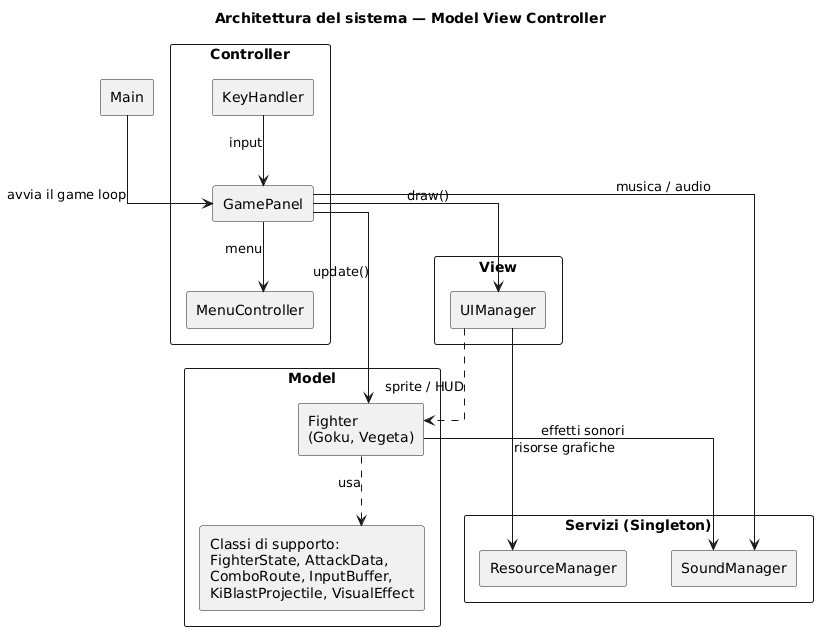
\includegraphics[width=.85\linewidth]{architettura}
  \caption{Architettura \emph{Model View Controller} (\emph{MVC}) dell'applicazione, con i moduli principali, i servizi infrastrutturali (\texttt{ResourceManager}, \texttt{SoundManager}) e le direzioni dei principali flussi informativi.}
  \label{fig:arch}
\end{figure}

Il cuore dell'esecuzione è il \emph{game loop} ospitato in \texttt{GamePanel}, che implementa l'interfaccia \texttt{Runnable} ed è eseguito su un \emph{thread} dedicato. Il \emph{loop} adotta un passo temporale fisso pari a $1/60$ di secondo: a ogni iterazione invoca il metodo \texttt{update()}, che fa avanzare la logica di gioco, e successivamente il metodo \texttt{repaint()}, che richiede il ridisegno della schermata; una fase di attesa calibrata mantiene la frequenza costante a 60 fotogrammi al secondo. Il ridisegno è delegato dal metodo \texttt{paintComponent()} di \texttt{GamePanel} alla \emph{View}, cioè alla classe \texttt{UIManager}.

Va precisato che la suddivisione descritta non costituisce una realizzazione ortodossa del pattern MVC. Poiché l'applicazione è basata su Swing, la classe \texttt{GamePanel} riveste un duplice ruolo: è al tempo stesso la superficie di disegno (in quanto estende \texttt{JPanel}) e il motore che ospita il ciclo di gioco. Inoltre, per ragioni di coesione, ogni personaggio conosce il modo in cui rappresentarsi a schermo, esponendo un proprio metodo di disegno. Si è preferito privilegiare la chiarezza e l'efficienza dell'implementazione rispetto a un'aderenza formale al pattern, mantenendone comunque i principi fondamentali: la logica di gioco è nettamente separata dall'input e la responsabilità del disegno delle schermate è concentrata in un unico modulo.

Nella progettazione ricorrono alcuni \emph{design pattern} che verranno richiamati nelle sezioni successive: il \emph{Singleton} per i servizi di gestione delle risorse e dell'audio; il \emph{Template Method} per la definizione del comportamento comune dei personaggi; una \emph{macchina a stati finiti} (\emph{Finite State Machine}) per governare le condizioni di ciascun personaggio; e l'impiego di \emph{oggetti immutabili} per la descrizione dei dati di combattimento.
% Architettura del Sistema Software [end]
%-------------------------------------------

% Model [start]
%-------------------------------------------
\section{Model}\label{se:arch.model}
Il \emph{Model} raccoglie lo stato dell'incontro e le regole del combattimento. La sua struttura è rappresentata nel diagramma delle classi di Fig.~\ref{fig:model}.

\begin{figure}[tb]
  \centering
  % TODO: inserire in figures/ il diagramma delle classi del Model (model-class-diagram.png)
  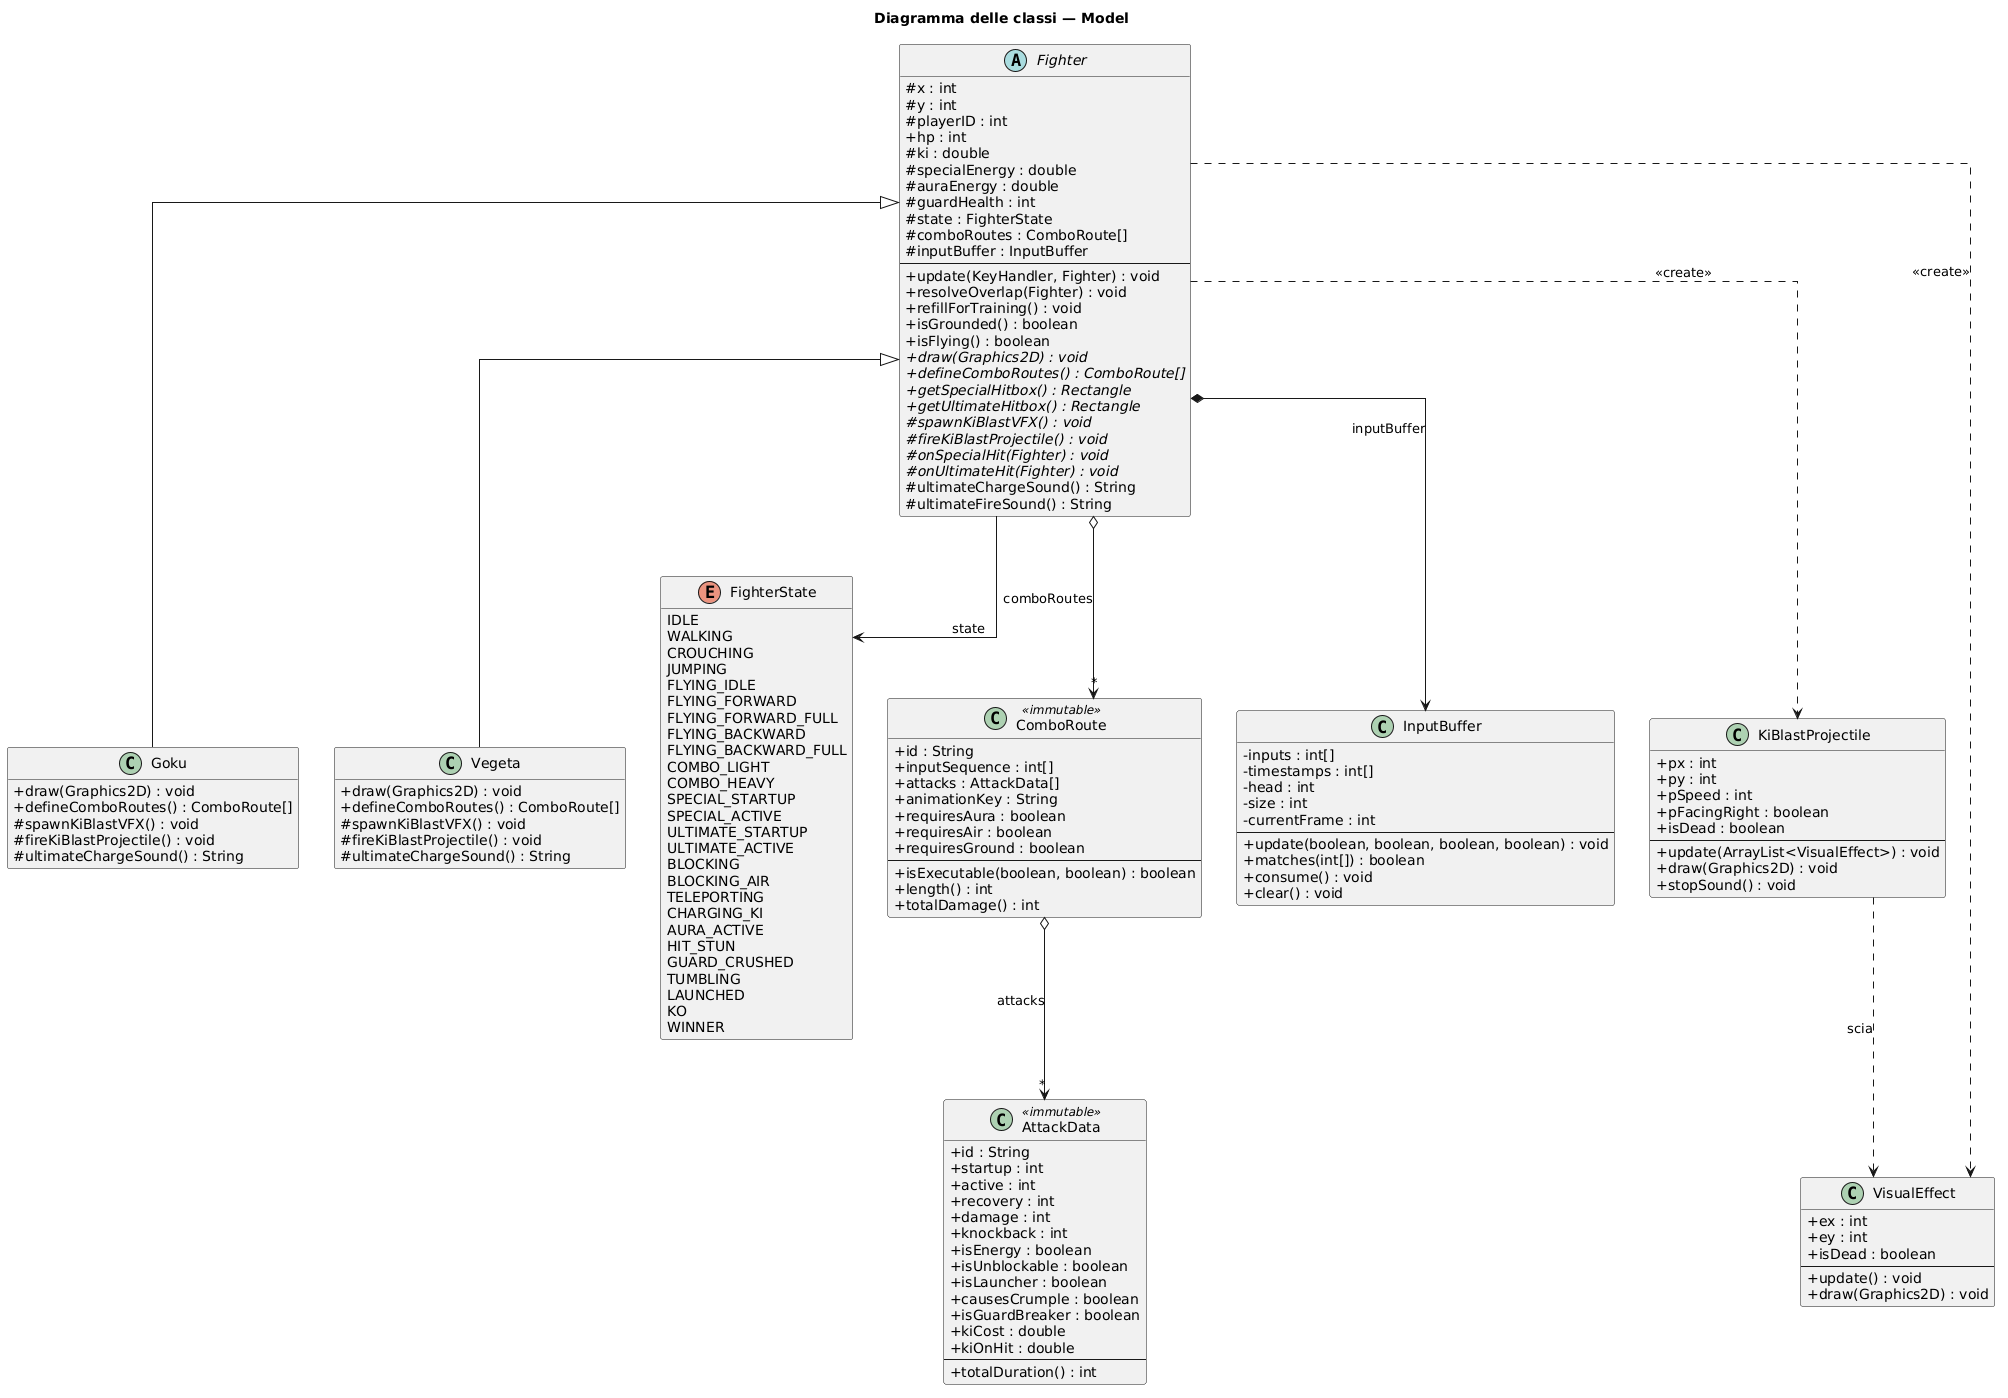
\includegraphics[width=\linewidth]{model-class-diagram}
  \caption{Diagramma delle classi del modulo \emph{Model}: la gerarchia \texttt{Fighter} e le classi di supporto per stati, combo e entità dinamiche.}
  \label{fig:model}
\end{figure}

L'elemento centrale del modulo è la classe astratta \texttt{Fighter}, che raccoglie tutto ciò che è comune ai personaggi: posizione, statistiche (punti vita, energia \emph{Ki}, cariche di speciale e aura), modello fisico per salto e gravità, sistema di combo, gestione della guardia e delle reazioni ai colpi. La classe applica il pattern \emph{Template Method}~\cite{gof}: il metodo \texttt{update(KeyHandler, Fighter)} costituisce lo scheletro invariante dell'aggiornamento di un personaggio a ogni fotogramma --- aggiornamento dei suoni di transizione, avanzamento degli effetti visivi e successiva gestione dipendente dallo stato corrente --- mentre i comportamenti specifici di ciascun personaggio sono demandati a un insieme di metodi astratti, sovrascritti dalle sottoclassi:
\begin{itemize}
  \item \texttt{draw(Graphics2D)} --- disegna lo \emph{sprite} del personaggio nello stato corrente;
  \item \texttt{defineComboRoutes()} --- restituisce l'insieme delle combo eseguibili dal personaggio;
  \item \texttt{getSpecialHitbox()}, \texttt{getUltimateHitbox()} --- forniscono le aree di collisione della mossa speciale e dell'ultimate;
  \item \texttt{spawnKiBlastVFX()}, \texttt{fireKiBlastProjectile()} --- generano rispettivamente l'effetto visivo di caricamento e il proiettile energetico;
  \item \texttt{onSpecialHit(Fighter)}, \texttt{onUltimateHit(Fighter)} --- definiscono gli effetti prodotti sull'avversario dai colpi energetici.
\end{itemize}
A questi si aggiungono i due metodi \texttt{ultimateChargeSound()} e \texttt{ultimateFireSound()}, che espongono l'effetto sonoro della mossa speciale e restituiscono un valore nullo nella classe base, in modo che ciascun personaggio possa specificarlo autonomamente. Le sottoclassi concrete \texttt{Goku} e \texttt{Vegeta} forniscono i parametri caratteristici (velocità, danno, costi in energia, durata di caricamento delle mosse) e l'implementazione dei metodi astratti, distinguendo così i due personaggi pur condividendo l'intera struttura di controllo.

Il comportamento di un personaggio è governato da una \emph{macchina a stati finiti}, i cui stati sono raccolti nell'enumerazione \texttt{FighterState}. Gli stati --- una ventina abbondante --- sono organizzati per categorie: stati di movimento (riposo, camminata, salto, volo nelle sue varianti), stati di combattimento (attacchi leggeri e pesanti, caricamento ed esecuzione di speciale e ultimate), stati di difesa (guardia a terra e in aria, teletrasporto), stati legati all'energia (carica del \emph{Ki}, aura attiva) e stati di reazione al danno (stordimento, guardia rotta, proiezione in aria). Il metodo \texttt{update()} seleziona, in base allo stato corrente, il blocco di logica da eseguire, realizzando così le transizioni tra le diverse condizioni del personaggio.

Attorno a \texttt{Fighter} ruotano alcune classi di supporto:
\begin{itemize}
  \item \texttt{AttackData} --- oggetto \emph{immutabile} che descrive un singolo colpo attraverso i suoi dati di temporizzazione (fotogrammi di \emph{startup}, di attività e di \emph{recovery}), il danno, la spinta (\emph{knockback}), il costo e la ricompensa in energia, e una serie di proprietà (colpo energetico, imblocabile, in grado di proiettare in aria o di rompere la guardia). Tutti i campi sono dichiarati \texttt{final} e valorizzati un'unica volta in costruzione; diversi costruttori sovraccarichi ne agevolano la creazione nei casi più comuni.
  \item \texttt{ComboRoute} --- anch'esso immutabile, rappresenta una combo come sequenza di input associata a un vettore di \texttt{AttackData}, a una chiave di animazione e a eventuali vincoli di esecuzione (con aura attiva, in aria o a terra); il metodo \texttt{isExecutable()} verifica se la combo è disponibile nella condizione corrente del personaggio.
  \item \texttt{InputBuffer} --- realizza il riconoscimento delle combo (\emph{Neo Combo}). Registra gli input recenti in un buffer circolare associando a ciascuno l'istante di pressione e adottando una logica di \emph{edge detection}, così da registrare la singola pressione e non il tasto mantenuto; il metodo \texttt{matches()} confronta gli ultimi input --- purché ancora entro una finestra temporale prestabilita --- con una sequenza attesa.
  \item \texttt{KiBlastProjectile} e \texttt{VisualEffect} --- rappresentano le entità dinamiche presenti sul campo, rispettivamente i proiettili energetici e gli effetti particellari. Vengono mantenute in apposite liste, aggiornate a ogni fotogramma e rimosse automaticamente al termine del loro ciclo di vita.
\end{itemize}
% Model [end]
%-------------------------------------------

% View [start]
%-------------------------------------------
\section{View}\label{se:arch.view}
La \emph{View} ha il compito di rappresentare a schermo lo stato dell'applicazione ed è concentrata nella classe \texttt{UIManager}, la cui struttura è illustrata in Fig.~\ref{fig:view}. Il metodo pubblico \texttt{draw(Graphics2D)} funge da dispatcher: in base allo stato corrente dell'applicazione, delega il disegno al metodo specializzato per la schermata attiva (schermata iniziale, caricamento, menu principale, selezione del personaggio, selezione dell'arena, schermata di presentazione dello scontro, incontro, comandi e crediti). Al di sopra di ogni schermata, a partire dal menu principale, viene sovrapposto l'indicatore di stato dell'audio.

\begin{figure}[tb]
  \centering
  % TODO: inserire in figures/ il diagramma delle classi della View (view-class-diagram.png)
  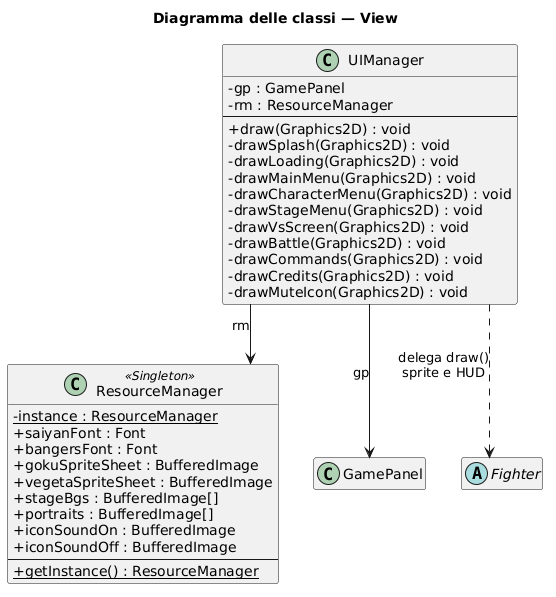
\includegraphics[width=\linewidth]{view-class-diagram}
  \caption{Diagramma delle classi del modulo \emph{View}: la classe \texttt{UIManager} e la sua relazione con il \texttt{ResourceManager} per l'accesso alle risorse grafiche.}
  \label{fig:view}
\end{figure}

Per il disegno, \texttt{UIManager} attinge alle risorse (\emph{sprite}, sfondi, icone, ritratti, \emph{font}) caricate una sola volta all'avvio dal \texttt{ResourceManager}. La responsabilità del disegno non è tuttavia interamente accentrata nella \emph{View}: in coerenza con quanto osservato in fase di architettura, ogni personaggio si disegna autonomamente tramite il proprio metodo \texttt{draw()}, e l'interfaccia di gioco (\emph{HUD}) --- barre dei punti vita, dell'energia, della carica speciale, dell'aura e della guardia, oltre ai ritratti e agli indicatori di combo --- è tracciata dal personaggio stesso. Durante l'incontro, pertanto, \texttt{UIManager} disegna lo sfondo dell'arena e coordina l'ordine di sovrapposizione (\emph{Z-index}) dei due contendenti, delegando ai personaggi il disegno dei rispettivi \emph{sprite} e della propria interfaccia. In Fig.~\ref{fig:screenshot-battle} e in Fig.~\ref{fig:screenshot-menu} sono riportate alcune schermate dell'applicazione.

\begin{figure}[tb]
  \centering
  % TODO: inserire in figures/ uno screenshot dell'incontro (screenshot-battle.png)
  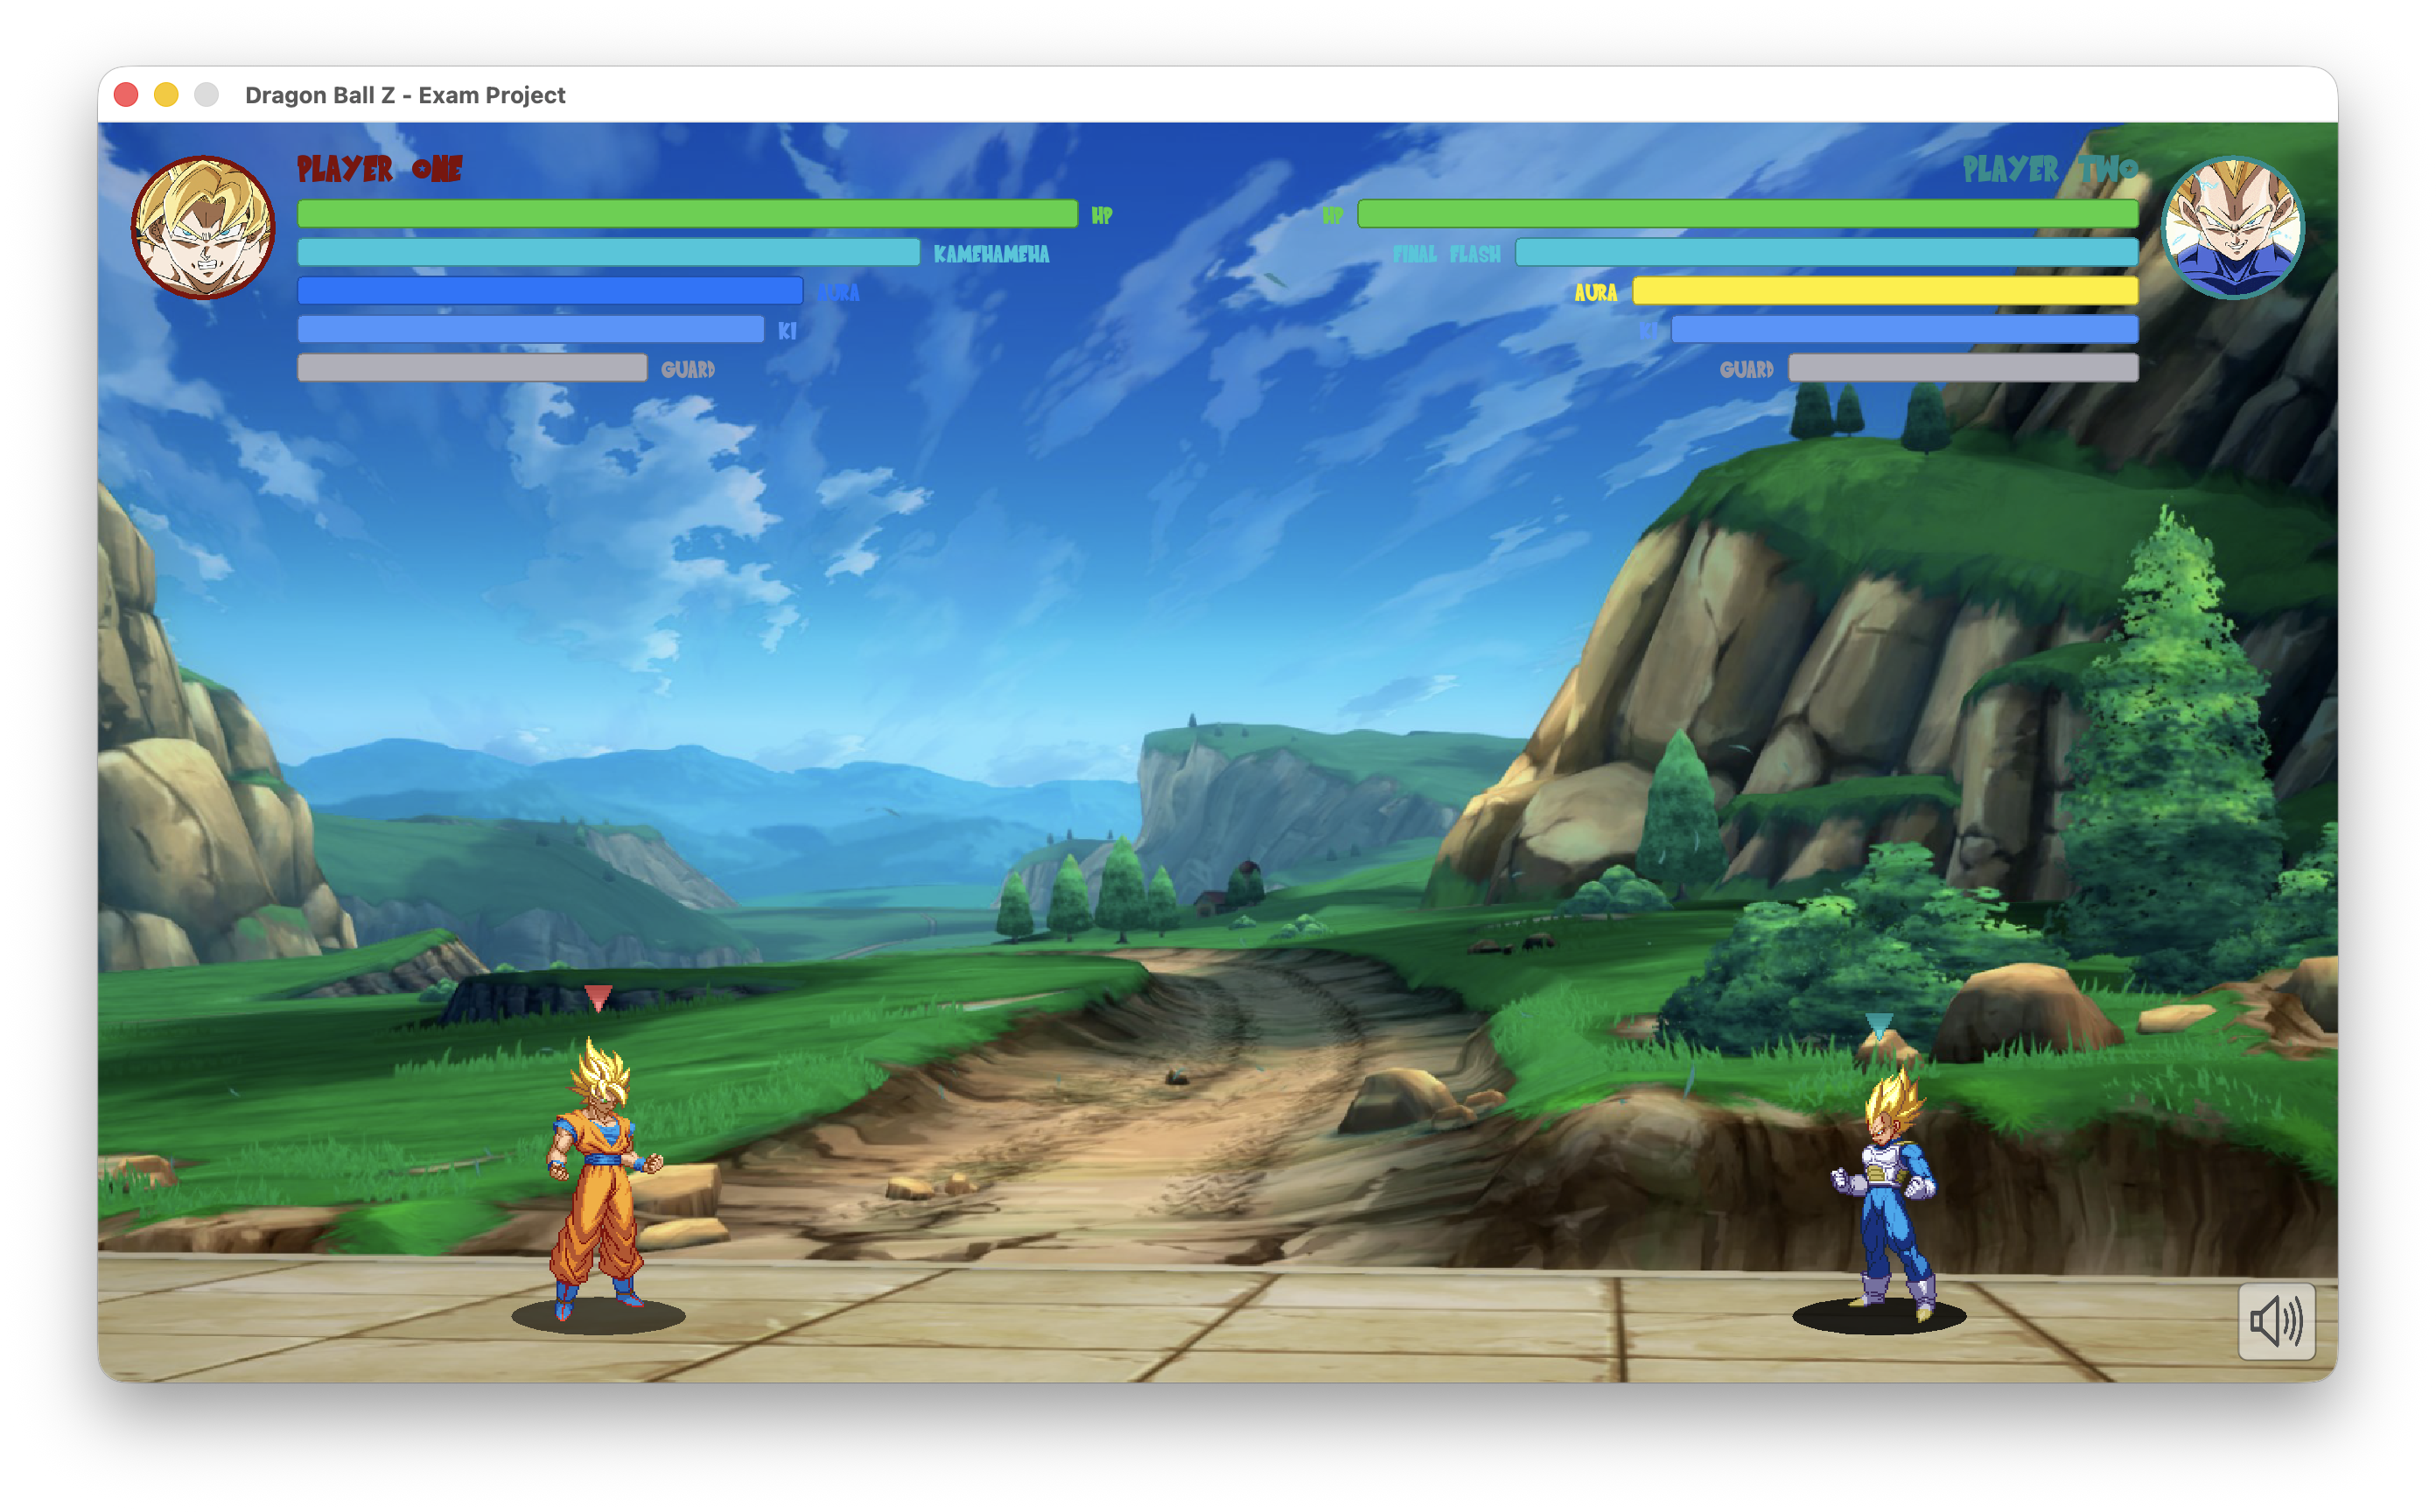
\includegraphics[width=.85\linewidth]{screenshot-battle}
  \caption{Schermata di combattimento: i due personaggi, gli effetti visivi e l'interfaccia di gioco (\emph{HUD}) con gli indicatori di punti vita, energia \emph{Ki}, carica speciale, aura e guardia.}
  \label{fig:screenshot-battle}
\end{figure}

\begin{figure}[tb]
  \centering
  % Screenshot del menu principale (screenshot-menu.png)
  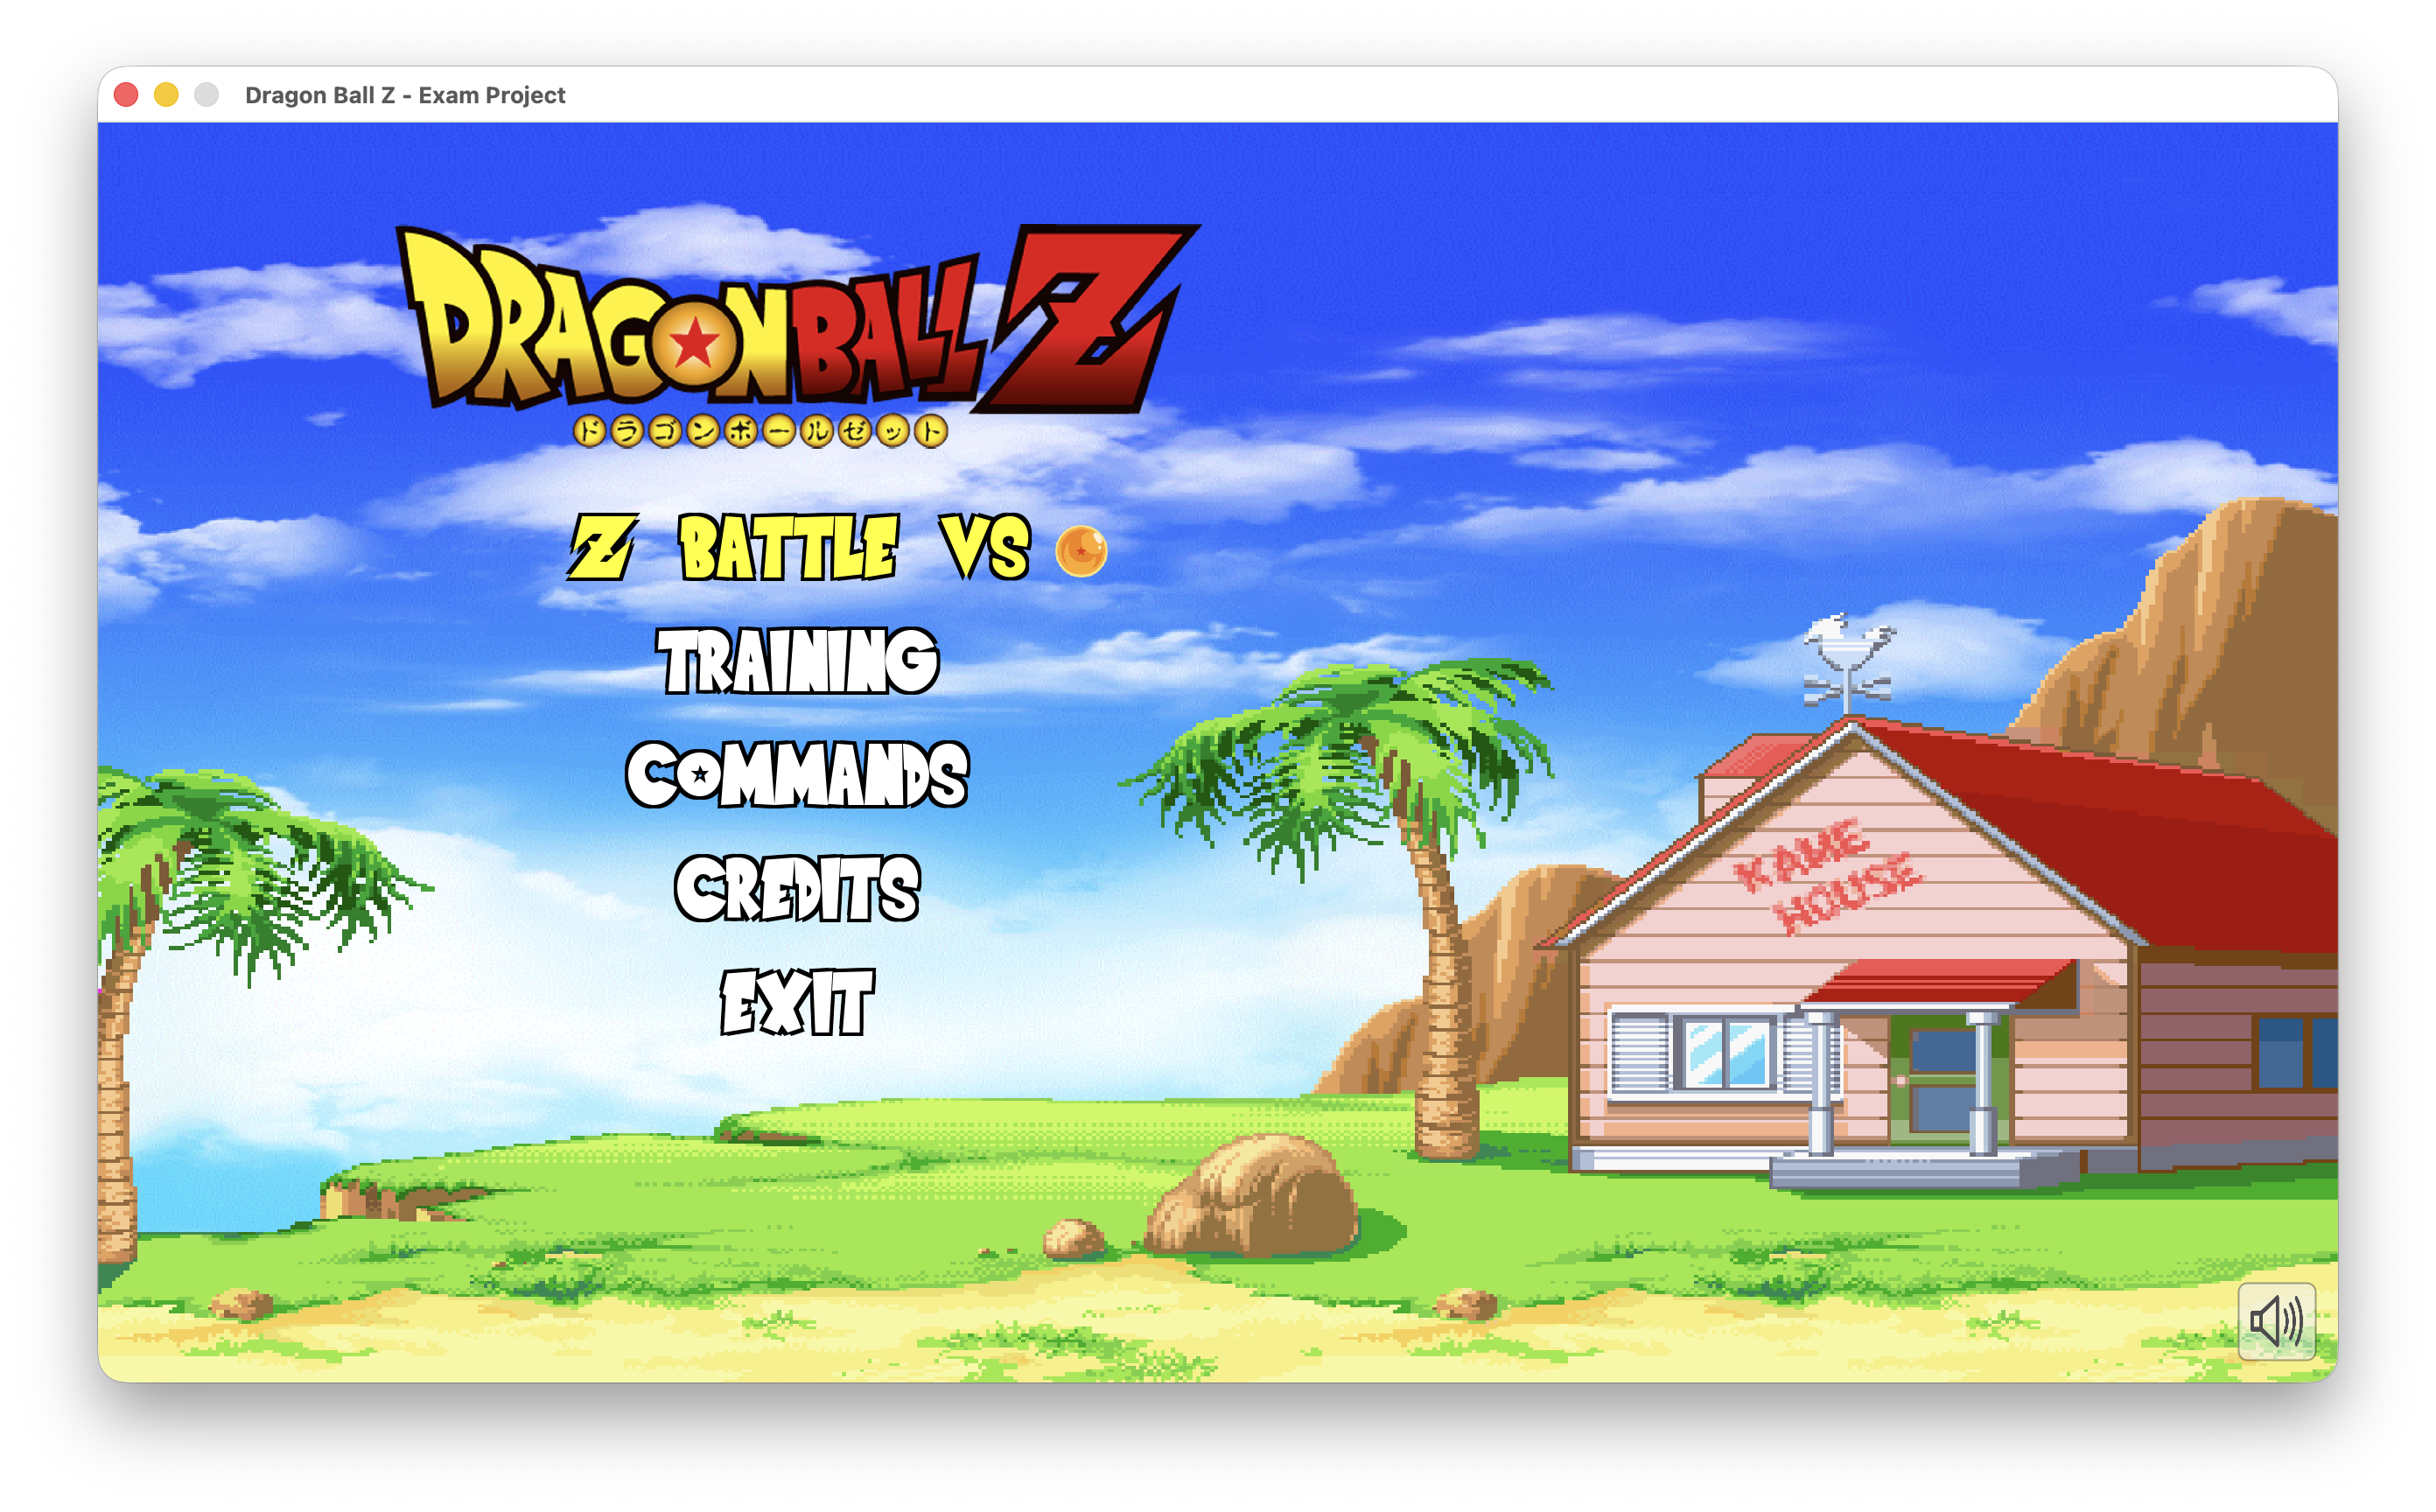
\includegraphics[width=.85\linewidth]{screenshot-menu}
  \caption{Schermata del menu principale, dalla quale si accede alla modalità di combattimento, alla modalità di addestramento e alle altre voci di navigazione.}
  \label{fig:screenshot-menu}
\end{figure}
% View [end]
%-------------------------------------------

% Controller [start]
%-------------------------------------------
\section{Controller}\label{se:arch.cont}
Il \emph{Controller} gestisce il flusso di esecuzione dell'applicazione e l'input dei giocatori. Esso è ripartito tra tre classi --- \texttt{GamePanel}, \texttt{MenuController} e \texttt{KeyHandler} --- la cui interazione è illustrata dal diagramma di sequenza di Fig.~\ref{fig:controller-seq}.

La classe \texttt{GamePanel} costituisce il motore dell'applicazione. Oltre a ospitare il \emph{game loop} descritto in precedenza, gestisce una \emph{macchina degli stati} dell'applicazione, che ne governa l'evoluzione attraverso le varie schermate (schermata iniziale, caricamento, menu, selezione, presentazione dello scontro, incontro). Durante l'incontro, un'ulteriore variabile di fase scandisce le sotto-fasi dello scontro: l'introduzione, il combattimento vero e proprio, la sconfitta di un contendente e la schermata di vittoria. A ogni fotogramma, nella fase di combattimento, \texttt{GamePanel} invoca l'aggiornamento dei due personaggi e ne rileva le collisioni per innescare, in proporzione alla violenza del colpo, l'effetto di tremolio dello schermo (\emph{screen shake}); coordina inoltre le transizioni di stato e i relativi segnali sonori.

\begin{figure}[tb]
  \centering
  % TODO: inserire in figures/ il diagramma di sequenza (controller-sequence.png)
  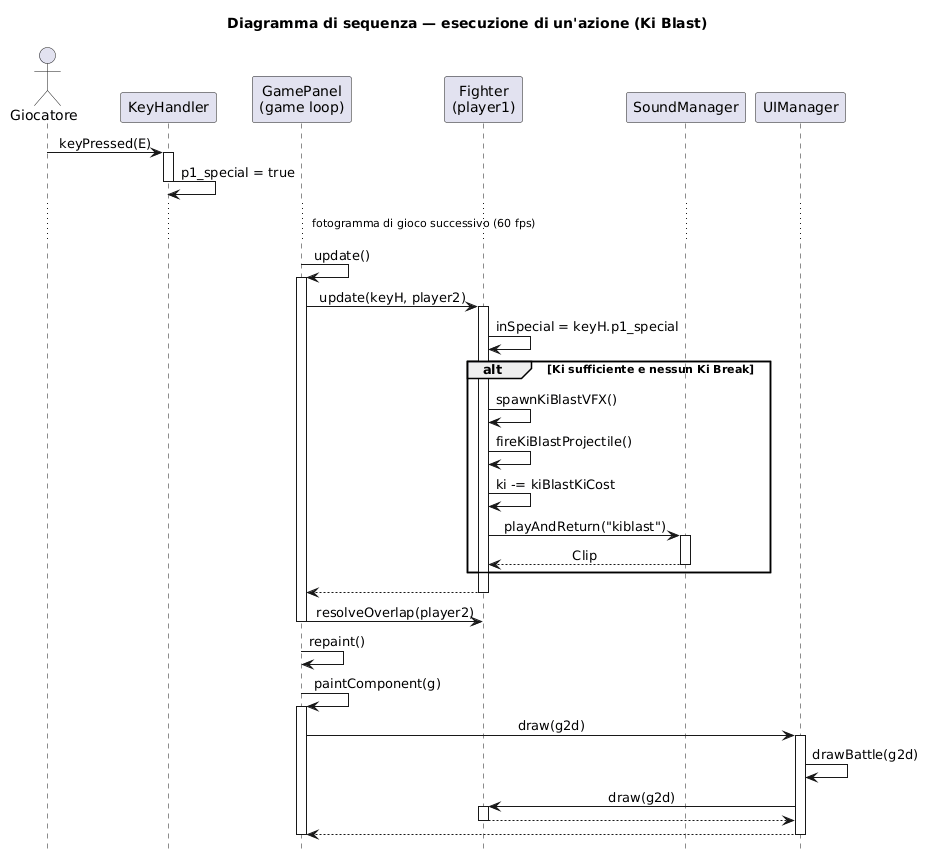
\includegraphics[width=.75\linewidth]{controller-sequence}
  \caption{Diagramma di sequenza che illustra la gestione di un'azione di gioco: dall'acquisizione dell'input da parte di \texttt{KeyHandler} all'aggiornamento del \emph{Model} e al conseguente ridisegno della schermata.}
  \label{fig:controller-seq}
\end{figure}

La classe \texttt{MenuController} incapsula la logica di navigazione dei menu. Per registrare correttamente le pressioni dei tasti direzionali e di conferma essa adotta una tecnica di \emph{edge detection}, confrontando lo stato dei tasti con quello del fotogramma precedente in modo da riconoscere il singolo evento di pressione e non il tasto mantenuto; in base all'input aggiorna la posizione dei cursori e provoca le transizioni tra le schermate.

La classe \texttt{KeyHandler} implementa l'interfaccia \texttt{KeyListener} e traduce gli eventi di pressione e rilascio dei tasti in un insieme di variabili booleane, distinte per i due giocatori e per il comando globale di disattivazione dell'audio. Essa non contiene alcuna logica di gioco: si limita a fotografare lo stato corrente della tastiera, che gli altri moduli interrogano quando necessario. La ripartizione dei comandi tra i due giocatori sulla medesima tastiera è dettagliata nella schermata dei comandi dell'applicazione.

La modalità di addestramento è realizzata riutilizzando integralmente il flusso di combattimento. La selezione dalla voce di menu attiva un indicatore in \texttt{GamePanel} che, durante l'incontro, mantiene costantemente al massimo i punti vita e le risorse di entrambi i personaggi (attraverso un metodo dedicato della classe \texttt{Fighter}) e disabilita la transizione verso la sconfitta, così che l'incontro non termini; il ritorno al menu avviene tramite un comando dedicato. Questa impostazione ha permesso di aggiungere la modalità senza duplicare la logica di combattimento e senza introdurre un avversario controllato dal calcolatore, coerentemente con l'assenza di intelligenza artificiale: nell'addestramento il secondo personaggio resta controllato dal secondo giocatore.
% Controller [end]
%-------------------------------------------

% Problemi Riscontrati [start]
%-------------------------------------------
\section{Problemi Riscontrati}\label{ch:proris}
Si riportano di seguito i principali problemi affrontati durante lo sviluppo, ovvero le difficoltà che hanno richiesto più tempo o che hanno imposto una revisione dell'impostazione adottata.

\begin{itemize}
  \item \textbf{Ripetizione spuria dell'effetto di volo.} L'effetto sonoro associato allo stacco da terra (salto o attivazione del volo) veniva erroneamente riprodotto ogni volta che il personaggio eseguiva un'azione (un attacco, un proiettile) mentre era in aria. La causa era nell'innesco del suono ``a livello'', cioè per tutta la durata della condizione di volo, anziché ``sulla transizione'', cioè nel solo istante del passaggio da terra ad aria. Il problema è stato risolto introducendo una condizione unificata che considera in volo il personaggio anche mentre esegue un'azione aerea, e confrontandola con lo stato del fotogramma precedente, così da innescare il suono una sola volta all'effettivo stacco.

  \item \textbf{Sincronizzazione della mossa speciale.} L'effetto sonoro delle mosse speciali (\emph{Kamehameha} e \emph{Final Flash}) contiene sia la fase di caricamento sia l'esplosione finale. Occorreva far coincidere l'apice sonoro dell'esplosione con la comparsa a schermo dell'onda energetica. Il risultato è stato ottenuto tarando per ciascun personaggio la durata di caricamento della mossa, in modo che l'onda parta esattamente quando il suono raggiunge il proprio culmine.

  \item \textbf{Esecuzione garantita dell'ultimate.} Per conferire alla mossa speciale il carattere spettacolare tipico del genere, si è reso necessario impedire che l'avversario potesse interromperla o sottrarsi ad essa. Si è quindi previsto che, durante l'esecuzione, l'avversario venga forzato in posizione di guardia e che la mossa risulti imblocabile, portandolo comunque in stato di stordimento se colpito.

  \item \textbf{Effetto di tremolio dello schermo.} L'effetto di \emph{screen shake} è realizzato traslando l'intera tela di disegno di uno scostamento casuale, proporzionale al \emph{knockback} del colpo, prima di disegnare la scena. Ha richiesto attenzione il ripristino della traslazione al termine del disegno: in sua assenza lo scostamento si sarebbe accumulato di fotogramma in fotogramma, facendo ``scivolare'' progressivamente l'intera scena.

  \item \textbf{Ridimensionamento dell'ambito del progetto.} In corso d'opera si è deciso di ridurre la portata del progetto per garantirne il completamento e la qualità entro i tempi previsti: il numero di personaggi giocabili è stato ricondotto a due (Goku e Vegeta) ed è stata rimossa una elaborata sequenza di ultimate cinematografica precedentemente abbozzata. L'infrastruttura per un \emph{roster} più ampio è stata comunque predisposta e lasciata inattiva, così da poter essere riattivata in sviluppi futuri.

  \item \textbf{Compenetrazione dei corpi.} Nelle prime versioni i due personaggi potevano occupare la medesima posizione --- atterrando uno sull'altro, uscendo dal volo o teletrasportandosi nello stesso punto --- e rimanevano di fatto incastrati, incapaci di muoversi. Il problema è stato risolto dotando ciascun personaggio di un corpo ``solido'' (\emph{pushbox}): quando due corpi si sovrappongono, un'apposita routine li allontana progressivamente. La separazione è attiva quando entrambi i personaggi sono a terra o in volo, mentre resta esclusa durante il salto, così da continuare a consentire lo scavalcamento dell'avversario; in aria viene inoltre verificata anche la sovrapposizione verticale, per non ostacolare chi vola a quote diverse.

  \item \textbf{Bilanciamento della guardia.} Nella prima stesura la difesa risultava troppo conveniente: parare un attacco fisico non comportava alcuna perdita di punti vita, e la barra della guardia, ampia e a rigenerazione rapida, era difficile da esaurire. Si è quindi rivisto il bilanciamento facendo sì che ogni parata lasci passare una quota ridotta del danno (senza però mai poter causare la sconfitta), riducendo la capienza della barra, aumentando il consumo per colpo parato e rallentandone il recupero, che riparte solo dopo un ritardo dall'ultima parata. La guardia resta così uno strumento efficace ma non più privo di controindicazioni.
\end{itemize}
% Problemi Riscontrati [stop]
%-------------------------------------------
%%%%%%%%%%%%%%%%%%%%%%%%%%
%     Progetto [end]     %
%%%%%%%%%%%%%%%%%%%%%%%%%%



%%%%%%%%%%%%%%%%%%%%%%%%%%%%%%%%%%%%%%%%%%%%%%%%%
%     Conclusioni e sviluppi futuri [start]     %
%%%%%%%%%%%%%%%%%%%%%%%%%%%%%%%%%%%%%%%%%%%%%%%%%
\chapter{Conclusioni e sviluppi futuri}\label{ch:conc-svil-fut}
Il lavoro svolto ha portato alla realizzazione di un videogioco di combattimento bidimensionale a due giocatori, completo tanto nella fase di combattimento quanto nel flusso di navigazione tra le schermate. Sono stati implementati un sistema di combo con concatenamento dei colpi, un sistema di proiettili e mosse speciali con gestione dell'energia, un potenziamento temporaneo, un sistema di difesa con guardia e teletrasporto, un insieme articolato di reazioni ai colpi e un comparto audio completo, oltre a una modalità di addestramento per la pratica libera, il tutto alla risoluzione di $1280 \times 720$ pixel e alla frequenza di 60 fotogrammi al secondo.

Sul piano progettuale, l'adozione di un'architettura ispirata al pattern MVC ha permesso di mantenere separate la logica di gioco, la sua visualizzazione e la gestione dell'input, agevolando lo sviluppo incrementale. Il ricorso al \emph{Template Method} nella gerarchia dei personaggi ha reso possibile condividere l'intera struttura di controllo tra Goku e Vegeta, delegando alle sottoclassi i soli aspetti caratteristici; la \emph{macchina a stati finiti} ha fornito un modello chiaro e verificabile per governare le numerose condizioni di ciascun personaggio; i due \emph{Singleton} di gestione delle risorse e dell'audio hanno centralizzato il caricamento degli \emph{asset} evitandone la duplicazione.

L'applicazione si presta a diverse estensioni. La più immediata è l'ampliamento del \emph{roster}: l'infrastruttura di selezione e di caricamento delle risorse è già predisposta per accogliere ulteriori personaggi, la cui aggiunta richiede la sola definizione delle corrispondenti sottoclassi di \texttt{Fighter}. Sono inoltre ipotizzabili l'introduzione di un avversario controllato dal calcolatore (\emph{intelligenza artificiale}), la reintroduzione della sequenza di ultimate cinematografica e un'ulteriore rifinitura del bilanciamento dei parametri di combattimento.
%%%%%%%%%%%%%%%%%%%%%%%%%%%%%%%%%%%%%%%%%%%%%%%
%     Conclusioni e sviluppi futuri [end]     %
%%%%%%%%%%%%%%%%%%%%%%%%%%%%%%%%%%%%%%%%%%%%%%%


%%%%%%%%%%%%%%%%%%%%%%%%%%%%%%%%%%%%%%%%%%%%%
%     Bibliografia e Sitografia [start]     %
%                 NO BibTeX                 %
%%%%%%%%%%%%%%%%%%%%%%%%%%%%%%%%%%%%%%%%%%%%%
%\chapter{Bibliografia e Sitografia}\label{ch:bibsit}
%
%\begin{thebibliography}{9}
%\bibitem{lamport94}
%  Leslie Lamport,
%  \textit{\LaTeX: a document preparation system},
%  Addison Wesley, Massachusetts,
%  2nd edition,
%  1994.
%\end{thebibliography}
%
%%%%%%%%%%%%%%%%%%%%%%%%%%%%%%%%%%%%%%%%%%%%
%     Bibliografia e Sitografia [end]     %
%                 NO BibTeX               %
%%%%%%%%%%%%%%%%%%%%%%%%%%%%%%%%%%%%%%%%%%%%



%%%%%%%%%%%%%%%%%%%%%%%%%%%%%%%%%%%%%%%%%%%%%
%     Bibliografia e Sitografia [start]     %
%                with BibTeX                %
%%%%%%%%%%%%%%%%%%%%%%%%%%%%%%%%%%%%%%%%%%%%%
\bibliographystyle{plain}
% Fonti delle risorse (immagini, suoni, font): elencate in bibliografia senza citarle nel testo
\nocite{sprites,audiofreesound,audiomyinstants,audiovoicy,fontsaiyan,fontbangers}
\bibliography{bibliografia}
% inserire i riferimenti bibliografici nel file 'bibliografia.bib'
%%%%%%%%%%%%%%%%%%%%%%%%%%%%%%%%%%%%%%%%%%%
%     Bibliografia e Sitografia [end]     %
%                with BibTeX              %
%%%%%%%%%%%%%%%%%%%%%%%%%%%%%%%%%%%%%%%%%%%



%%%%%%%%%%%%%%%%%%%%%%%%%%%%%
%     Appendice [start]     %
%%%%%%%%%%%%%%%%%%%%%%%%%%%%%
\chapter{Appendice}\label{ch:app}

\section{Attribuzione delle risorse}
Gli \emph{asset} grafici e sonori impiegati nell'applicazione --- \emph{sprite} dei personaggi e degli stage, effetti visivi, effetti sonori e tracce musicali --- derivano dalla serie animata e dai videogiochi di \emph{Dragon Ball Z}, di proprietà dei rispettivi detentori dei diritti (Bandai Namco Entertainment, Toei Animation, Akira Toriyama e Shueisha). Tali materiali sono stati utilizzati esclusivamente a scopo didattico, nell'ambito del corso di Programmazione di Interfacce Grafiche e Dispositivi Mobili, e senza alcuna finalità di lucro. Le fonti da cui i singoli asset sono stati reperiti --- gli \emph{sprite}, gli effetti sonori, le tracce musicali e i \emph{font} --- sono elencate nella bibliografia.

\section{Estratti di codice}
Si riportano di seguito due estratti significativi del codice sorgente. Il primo (Listato~\ref{lst:gameloop}) mostra il \emph{game loop} a passo fisso che governa l'intera esecuzione; il secondo (Listato~\ref{lst:pushbox}) mostra la routine di separazione dei corpi discussa nella Sezione~\ref{ch:proris}.

\begin{lstlisting}[style=java, caption={Il \emph{game loop} a 60 fotogrammi al secondo (\texttt{GamePanel.run()}).}, label=lst:gameloop]
@Override
public void run() {
    double drawInterval = 1000000000.0 / FPS; // durata di un fotogramma (ns)
    double nextDrawTime = System.nanoTime() + drawInterval;

    while (gameThread != null) {
        update();   // avanza la logica di gioco
        repaint();  // richiede il ridisegno della schermata

        try {
            double remainingTime = (nextDrawTime - System.nanoTime()) / 1000000;
            if (remainingTime < 0) remainingTime = 0;
            Thread.sleep((long) remainingTime); // mantiene i 60 fps
            nextDrawTime += drawInterval;
        } catch (InterruptedException e) { e.printStackTrace(); }
    }
}
\end{lstlisting}

\begin{lstlisting}[style=java, caption={La separazione dei corpi sovrapposti (\texttt{Fighter.resolveOverlap()}).}, label=lst:pushbox]
public void resolveOverlap(Fighter other) {
    // Attivo solo se entrambi sono a terra o in volo (il salto resta libero)
    if (!canBePushed() || !other.canBePushed()) return;

    // Sovrapposizione orizzontale e verticale dei due corpi
    int overlapX = Math.min(x + baseWidth, other.x + other.baseWidth)
                 - Math.max(x, other.x);
    if (overlapX <= 0) return;
    int overlapY = Math.min(y + baseHeight, other.y + other.baseHeight)
                 - Math.max(y, other.y);
    if (overlapY <= 0) return;

    // Allontanamento: meta' spostamento a testa, limitato
    int push = Math.min((overlapX + 1) / 2, MAX_SEPARATION_PUSH);
    int thisCenter  = x + baseWidth / 2;
    int otherCenter = other.x + other.baseWidth / 2;
    boolean thisIsLeft = (thisCenter < otherCenter)
            || (thisCenter == otherCenter && playerID < other.playerID);

    if (thisIsLeft) { x -= push; other.x += push; }
    else            { x += push; other.x -= push; }

    clampX();
    other.clampX();
}
\end{lstlisting}
%%%%%%%%%%%%%%%%%%%%%%%%%%%
%     Appendice [end]     %
%%%%%%%%%%%%%%%%%%%%%%%%%%%



\end{document}
%%%%%%%%%%%%%%%%%%%%%%%%%%%%%%%%
%                              %
%     Begin Docuemnt [end]     %
%                              %
%%%%%%%%%%%%%%%%%%%%%%%%%%%%%%%%